\begin{figure*}[t]
    \centering
    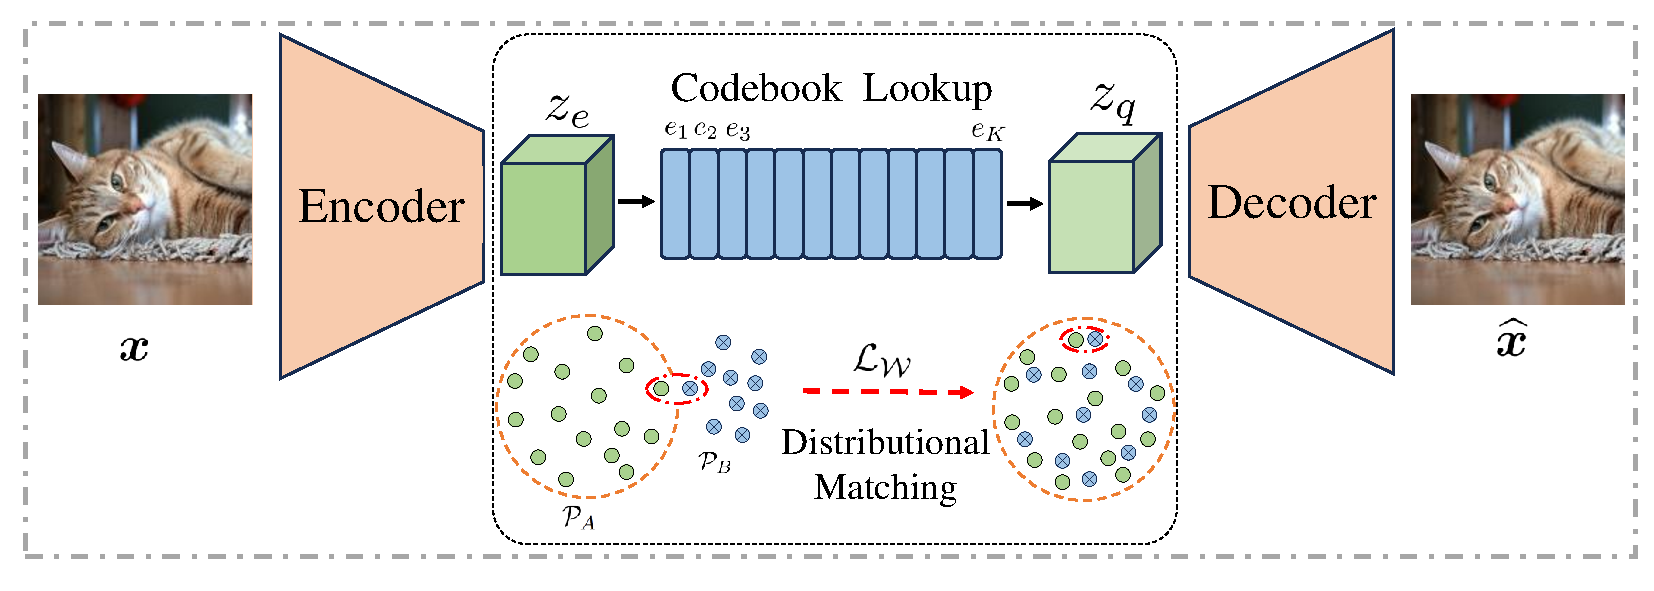
\includegraphics[width=0.86\linewidth]{figs/architecture/WassersteinVQ_new.pdf}
    \vspace{-3ex}
    \caption{\small{Illustration of the \emph{Wasserstein VQ}. The architecture integrates an encoder-decoder network with a  VQ module. In the VQ module, we augment the vanilla VQ framework~\citep{Oord2017NeuralDR} by incorporating our proposed Wasserstein loss $\mathcal{L}_{\mathcal{W}}$ to achieve distributional matching between features $\bz_e$ ($\bz_e^{ij}\sim \mathcal{P}_{A}$) and the codebook $\be_k$ ($\be_k\sim \mathcal{P}_{B}$).}}
    \label{fig:wasserstein vq}
    \vspace{-3ex}
\end{figure*}

\section{Methodology}
\label{sec:method}

% In this section, we introduce the quadratic Wasserstein distance for distributional matching between features and the codebook. We then apply this technique to two frameworks.

\textcolor{red}{In this section, we instantiate the distributional alignment principle developed in Section~\ref{sec:understanding} using a Wasserstein-based objective. We then integrate this objective into two representative vector quantization frameworks.}

\textcolor{blue}{Based on the theoretical insights in Section~\ref{sec:understanding}, we propose a general framework for enhancing Vector Quantization via distributional matching. We first formulate the general objective and then present two distinct instantiations: a parametric approach using Wasserstein distance and a non-parametric alternative using Maximum Mean Discrepancy (MMD).}

\textcolor{green}{Based on the theoretical insights in Section~\ref{sec:understanding}, 
we propose a general framework for enhancing vector quantization via distributional matching, 
which can be instantiated using either parametric objectives (e.g., Wasserstein distance) 
or non-parametric alternatives (e.g., maximum mean discrepancy). We then integrate this objective into two representative vector quantization frameworks.}

\textcolor{blue}{\subsection{The Distributional Matching Framework}
To resolve the fundamental mismatch between the feature distribution $\mathcal{P}_A$ and the codebook distribution $\mathcal{P}_B$, we introduce an auxiliary alignment loss $\mathcal{L}_{match}$ to the standard VQ objective. The goal is to minimize the divergence $\mathcal{D}$ between the two distributions:
\begin{equation}
    \mathcal{L}_{match} = \mathcal{D}(\mathcal{P}_A, \mathcal{P}_B),
\end{equation}
where $\mathcal{P}_A$ is empirically defined by the encoder outputs $\{\bm{z}_e\}$ and $\mathcal{P}_B$ by the code vectors $\{\bm{e}_k\}$. Crucially, gradients from $\mathcal{L}_{match}$ are only back-propagated to the codebook, ensuring that the feature expressiveness of the encoder remains unaffected.
}

\textcolor{blue}{\subsection{Instantiation I: Efficient Matching via Wasserstein Distance}\label{sec:wasserstein}
We first consider a parametric instantiation assuming a mild Gaussian approximation for computational efficiency. We model both distributions as multivariate Gaussians, i.e., $\mathcal{P}_A \approx \mathcal{N}(\bm{\mu}_1, \bm{\Sigma}_1)$ and $\mathcal{P}_B \approx \mathcal{N}(\bm{\mu}_2, \bm{\Sigma}_2)$. Under this assumption, we employ the quadratic Wasserstein distance, as defined in Appendix~\ref{appendix: distribution distance}, which admits a computationally efficient closed-form solution. 
}

\subsection{Wasserstein-Based Distribution Matching}
\label{sec:wasserstein distance}

We assume a Gaussian hypothesis for the distributions of both the feature and code vectors. For computational efficiency, we employ the quadratic Wasserstein distance, as defined in Appendix~\ref{appendix: distribution distance},  to align these two distributions. 

Although other statistical distances, such as the Kullback-Leibler divergence \citep{Kingma2013AutoEncodingVB, Ho2020DenoisingDP}, are viable alternatives, they lack simple closed-form representations, making them computationally expensive. The following lemma provides the closed-form representation for the quadratic Wasserstein distance between two Gaussian distributions.  

\begin{lemma}[\citep{Olkin1982TheDB}]\label{theorem:Wasserstein Distance}
The quadratic Wasserstein distance between $\mathcal{N}(\bm \mu_1, \m \Sigma_1)$ and $\mathcal{N}(\bm \mu_2, \m \Sigma_2)$ 
\begin{equation}\label{eq:wasserstein distance definition}
\sqrt{\Vert \bm \mu_1 - \bm \mu_2 \Vert^2_2 + \tr( {\m \Sigma_1}+ {\m \Sigma_2} - 2 (\Sigma_1^{\frac{1}{2}} {\m \Sigma_2} \m \Sigma_1^{\frac{1}{2}})^{\frac{1}{2}})}.
\end{equation}
\end{lemma}
\textcolor{red}{The lemma shows that the quadratic Wasserstein distance admits a closed-form expression in terms of the means and covariance matrices of the two distributions.
}
% The lemma above indicates that the quadratic Wasserstein distance can be easily computed using the population means and covariance matrices. 
In practice, we estimate these population quantities, ${\bm \mu}_{1}$, ${\bm \mu}_{2}$, ${\m \Sigma}_{1}$, and ${\m \Sigma}_{2}$, with their sample counterparts: $\hat {\bm \mu}_{1}$, $\hat {\bm \mu}_{2}$, $\hat {\m \Sigma}_{1}$, and $\hat {\m \Sigma}_{2}$. 
The empirical quadratic Wasserstein distance is then used as the optimization objective to align  the feature and codebook distributions:
\begin{equation}\label{eq:wasserstein distance}
\mathcal{L}_{\mathcal{W}}\! = \!\sqrt{\!\Vert \hat {\bm \mu}_{1} \!- \!\hat {\bm \mu}_{2} \Vert^2_2 \!+\! \tr( \hat {\m \Sigma}_{1}\!+\!\hat {\m \Sigma}_{2}\! -\!2(\hat {\m \Sigma}_{1}^{\frac{1}{2}} {\hat {\m \Sigma}_{2}} \hat {\m \Sigma}_{1}^{\frac{1}{2}})^{\frac{1}{2}})}. \nonumber
\end{equation}  
A smaller value of $\mathcal{L}_{\mathcal{W}}$ indicates stronger alignment  between the feature distribution $\mathcal{P}_A$ and the codebook  distribution $\mathcal{P}_B$. We refer to the VQ algorithm that employs $\mathcal{L}_{\mathcal{W}}$ as \emph{Wasserstein VQ}.

\paragraph{Remark.} Using $\mathcal{L}_{\mathcal{W}}$ does not reduce feature expressiveness, as it does not impose a Gaussian constraint on the underlying feature distribution. First, the Gaussian approximation is introduced solely to derive a closed-form expression for the Wasserstein loss, simplifying the complex form in Definition~\ref{def:wasserstien distance} in Appendix~\ref{appendix: distribution distance} into Lemma~\ref{theorem:Wasserstein Distance}. Second, this simplification does not affect the actual feature distribution, since $\mathcal{L}_{\mathcal{W}}$ is detached from the encoder; gradients of the Wasserstein distance update only the codebook parameters, leaving the feature representations unchanged. Third, in practice, the learned latent features in visual tokenization tasks often exhibit an approximately multivariate normal distribution. This tendency is not merely an assumption of Gaussianity; rather, it arises naturally from the aggregation of many weakly dependent components in deep representations, a behavior broadly consistent with the Central Limit Theorem (CLT). Such distributions are also information-theoretically favorable, as they maximize the entropy for a given covariance, thereby supporting efficient information transmission and robust signal reconstruction. Consequently, multivariate normal distributions emerge as an ideal and practically observed form for latent representations in visual tokenization and related signal recovery tasks.

\textcolor{blue}{\paragraph{Remark.}
The Gaussian approximation is introduced solely to obtain a closed-form and computationally efficient Wasserstein objective. Importantly, this approximation does not constrain the learned feature distribution: the Wasserstein loss $\mathcal{L}_{\mathcal{W}}$ is applied only to update the codebook parameters, while gradients to the encoder are detached. In practice, latent features in visual tokenization often exhibit approximately Gaussian statistics, a tendency commonly observed in deep representations. Moreover, in Section~\ref{sec:ablation} we show that replacing $\mathcal{L}_{\mathcal{W}}$ with a nonparametric alternative based on MMD yields comparable performance, indicating that the effectiveness of our approach does not hinge on the Gaussian assumption.}

\textcolor{green}{\paragraph{Remark on the Gaussian Assumption.} 
The Gaussian approximation is introduced solely to derive a closed-form and computationally efficient Wasserstein objective\textbf{, avoiding the expensive pair-wise computations required by non-parametric metrics.}
Importantly, this approximation does not constrain the learned feature expressiveness: the Wasserstein loss $\mathcal{L}_{W}$ is applied only to update the codebook parameters, while gradients to the encoder are detached. 
In practice, latent features in visual tokenization often exhibit approximately Gaussian statistics\textbf{, a behavior consistent with the Central Limit Theorem in high-dimensional deep representations.}
Moreover, as we demonstrate in Section~\ref{sec:mmd}, replacing $\mathcal{L}_{W}$ with a non-parametric alternative based on MMD yields comparable performance. 
\textbf{This confirms that the effectiveness of our distributional matching framework does not hinge on the Gaussian assumption, but rather on the alignment of distributions itself.}
}

%Third, in practice, an approximately Gaussian distribution can be observed in the learned latent features, which appears to emerge naturally from the aggregation of many weakly dependent components in deep representations, a phenomenon broadly consistent with the Central Limit Theorem (CLT), rather than being a consequence of our Gaussian hypothesis.

\textcolor{blue}{\subsection{Instantiation II: Robust Matching via MMD}\label{sec:mmd}
To address scenarios where the Gaussian assumption may not hold (e.g., highly multi-modal distributions), we provide a non-parametric instantiation using Maximum Mean Discrepancy (MMD)~\citep{gretton2012kernel}. MMD measures the distance between distributions in a Reproducing Kernel Hilbert Space (RKHS) without assuming any specific parametric form:
\begin{equation}
\mathcal{L}_{\text{MMD}} = \frac{1}{N^2}\sum_{i,j} k(\bm{z}_i, \bm{z}_j) - \frac{2}{NK}\sum_{i,k} k(\bm{z}_i, \bm{e}_k) + \frac{1}{K^2}\sum_{k,l} k(\bm{e}_k, \bm{e}_l),
\end{equation}
where $k(\cdot, \cdot)$ is a kernel function (e.g., Gaussian RBF kernel). 
While $\mathcal{L}_{\text{MMD}}$ offers greater theoretical robustness by relaxing the Gaussian hypothesis, it typically incurs a higher computational cost ($\mathcal{O}((N+K)^2)$) compared to the closed-form Wasserstein distance. In our experiments, we find that Wasserstein VQ yields performance comparable to MMD VQ (see Sec. 5), suggesting that the Gaussian approximation captures the essential structure for effective tokenization while remaining efficient.
}

\textcolor{red}{\subsection{Integration into VQ Architectures}
Our distributional matching framework is agnostic to the underlying VQ architecture. We integrate it into two representative frameworks: VQ-VAE and VQGAN.}

% \subsection{Integration into the VQ-VAE Framework}
\subsubsection{VQ-VAE Integration} 
\label{sec:VQVAE}
We first examine \emph{Wasserstein VQ} within the VQ-VAE framework~\citep{Oord2017NeuralDR}. As shown in Figure~\ref{fig:wasserstein vq}, the VQ-VAE model has three key components: an encoder $E(\cdot)$, a decoder $D(\cdot)$, and a quantizer $\mathcal{Q}(\cdot)$ with a learnable codebook $\{\m e_k\}_{k=1}^{K}$. As described earlier in Section~\ref{sec:overview vq}, for an input image $\bm{x}$, the encoder produces a spatial feature $\bm{z}_e = E(\bm{x}) \in \mathbb{R}^{h\times w \times d}$. The quantizer maps $\bm{z}_e$ to a quantized feature $\bm{z}_q$, which the decoder uses to reconstruct the image as $\bm{\hat{x}} = D(\bm{z}_q)$. Incorporating our Wasserstein loss $\mathcal{L}_{\mathcal{W}}$ into the VQ-VAE framework, the overall loss is formulated as follows:
\begin{align}
\label{eq:vqvae}
\mathcal{L}_{\text{VQ-VAE}} =\| \bm{\hat{x}} - \bm{x} \|^{2}_2 & + \beta \| \textrm{sg}(\bm{z}_q)-\bm{z}_e \|^{2}_2 \\\nonumber
 & + \| \textrm{sg}(\bm{z}_e) -\bm{z}_q \|^{2}_2 + \gamma \mathcal{L}_{\mathcal{W}}.
\end{align} 
where $\textrm{sg}$ denotes the stop-gradient. $\beta$ and $\gamma$ are hyper-parameters. We set $\gamma=0.5$ for all VQ-VAE experiments.

\textcolor{red}{By incorporating $\mathcal{L}_{\mathcal{W}}$, the codebook is encouraged to globally match the first- and second-order statistics of the feature distribution, complementing the local assignment enforced by the standard VQ loss.}

\paragraph{Remark.} 
Sections~\ref{sec:effects of distribution matching} and~\ref{sec:theoretical analysis} provide empirical and theoretical evidence that minimizing quantization error is closely linked to aligning the codebook with the feature distribution. By encouraging the codebook to reflect the feature space structure and density, the alignment loss $\mathcal{L}_{\mathcal{W}}$ positions code vectors as cluster centers, minimizing the average squared distance between feature vectors and their assigned codes, $\| \bm{z}_e - \bm{z}_q \|^{2}_2$. In essence, distribution alignment arranges prototypes to cover the feature manifold and fill gaps, reducing overall quantization error.

%Sections~\ref{sec:effects of distribution matching} and~\ref{sec:theoretical analysis} provide empirical and theoretical evidence that minimizing quantization error is closely linked to aligning the codebook distribution with that of the features. By encouraging the codebook to reflect the structure and density of the feature space, the alignment loss $\mathcal{L}_{\mathcal{W}}$ positions code vectors effectively as cluster centers, minimizing the average squared distance between feature vectors and their assigned codes, i.e., $\| \bm{z}_e - \bm{z}_q \|^{2}_2$. In essence, distribution alignment strategically arranges the prototypes to cover the feature manifold and fill gaps, thereby reducing overall quantization error.



\subsubsection{VQGAN Integration}
\label{sec:VQGAN}
To ensure high perceptual quality in the reconstructed images, we further investigate \emph{Wasserstein VQ} within the VQGAN framework~\citep{Esser2020TamingTF}. VQGAN extends the VQ-VAE framework by integrating a VGG network~\citep{Simonyan2014VeryDC}  and a patch-based discriminator \citep{Esser2020TamingTF, Johnson2016PerceptualLF}. The overall training objective of VQGAN can be written as follows:
\begin{align}
\label{eq:vqgan}
\mathcal{L}_{\text{VQGAN}} = \mathcal{L}_{\text{VQ-VAE}} + \mathcal{L}_{\text{Per}} + \lambda \mathcal{L}_{\text{GAN}}.
\vspace{-2ex}
\end{align}
%Where $\mathcal{L}_{\text{Per}}$ and $\mathcal{L}_{\text{GAN}}$ denote the VGG-based perceptual loss~\citep{Zhang2018TheUE}, and GAN loss~\citep{Isola2016ImagetoImageTW, Lim2017GeometricG}, respectively. Typically, achieving state-of-the-art reconstruction fidelity via adversarial training requires substantial computational resources. To mitigate training costs, we adopt the VQ-Transplant framework, which achieves competitive reconstruction fidelity at a fraction of the computational expense~\citep{Fang2025VQTransplant}. Specially, it initializes the encoder and decoder with a state-of-the-art pretrained tokenizer (e.g., VAR~\citep{Tian2024VisualAM}) instead of training from scratch, thereby significantly reducing training cost while maintaining reconstruction quality.
Where $\mathcal{L}_{\text{Per}}$ and $\mathcal{L}_{\text{GAN}}$ denote the VGG-based perceptual loss~\citep{Zhang2018TheUE} and the GAN loss~\citep{Isola2016ImagetoImageTW, Lim2017GeometricG}, respectively. Achieving state-of-the-art reconstruction fidelity via adversarial training typically incurs substantial computational cost. 
To reduce training overhead, we adopt the VQ-Transplant framework, which attains competitive reconstruction fidelity at a fraction of the cost~\citep{Fang2025VQTransplant}. 
\textcolor{red}{We adopt the VQ-Transplant framework solely as a training-efficient backbone; the proposed Wasserstein VQ is orthogonal to this choice and can be integrated into standard VQGAN training as well.}
Specifically, it initializes the encoder and decoder from a state-of-the-art pretrained tokenizer (e.g., VAR~\citep{Tian2024VisualAM}) rather than training from scratch, significantly lowering training cost while preserving reconstruction quality.

%which achieves competitive reconstruction fidelity at a fraction of the computational expense~\citep{Fang2025VQTransplant}. Within this framework, a frozen DINO-S~\citep{Caron2021EmergingPI,Oquab2023DINOv2LR} discriminator is employed, featuring an architecture similar to that of StyleGAN~\citep{Karras2019AnalyzingAI, karras2019style}. Following the original VQ-Transplant implementation~\citep{Fang2025VQTransplant}, we integrate DiffAug~\citep{Zhao2020DifferentiableAF}, consistency regularization~\citep{Zhang2019ConsistencyRF}, and LeCAM regularization~\citep{Tseng2021RegularizingGA} to train the discriminator. 



%The adaptive weight $\lambda_t$ is dynamically adjusted during training based on the gradient of the input with respect to the last layer of the decoder, following~\citep{Esser2020TamingTF}.